\chapter{La función de pérdida}
\label{cap:perdida}

\begin{enpocas}
Un solo número que diga qué tan mal lo hizo la red: clase, caja y distancias, en
dos cabezas que se combinan con un peso que cambia (ProgLoss). Archivos:
\cod{red_fuego/perdida.py} y \cod{red_fuego/perdida_iou.py}.
\end{enpocas}

\section{Tres términos por cabeza}

Una vez asignadas las celdas, cada cabeza calcula
\begin{equation}
L = 7.5\,L_{\text{caja}} + 0.5\,L_{\text{clase}} + 1.5\,L_{\text{dist}},
\end{equation}
con las ganancias por omisión de Ultralytics. Sea $\Omega$ el conjunto de celdas
positivas, $\hat t_i$ el objetivo suave de la celda $i$
(capítulo~\ref{cap:asignacion}) y $S = \sum_i \hat t_i$.

\subsection{Clase: entropía cruzada binaria}
En \emph{todas} las celdas y para cada clase $c$:
\begin{equation}
L_{\text{clase}} = \frac{1}{S}\sum_{i}\sum_{c} -\big[\hat t_{ic}\log\sigma(z_{ic})
+ (1-\hat t_{ic})\log(1-\sigma(z_{ic}))\big].
\end{equation}
Las celdas de fondo tienen $\hat t = 0$ y aprenden a decir «nada». Se usa una
sigmoide por clase (no un \emph{softmax}) porque fuego y humo pueden aparecer en
la misma celda.

\subsection{Caja: CIoU}
\paso{15} \textbf{Escribir \cod{ciou}.}
El IoU mide el traslape entre la caja predicha $B$ y la real $B^\ast$, pero vale
cero cuando no se tocan y entonces no da gradiente. CIoU (\emph{Complete IoU}) le
resta dos castigos:
\begin{equation}
\mathrm{CIoU} = \mathrm{IoU} - \frac{\rho^2(\mathbf{c},\mathbf{c}^\ast)}{d^2} - \alpha v,
\qquad v = \frac{4}{\pi^2}\Big(\arctan\frac{w^\ast}{h^\ast} - \arctan\frac{w}{h}\Big)^2,
\end{equation}
donde $\rho$ es la distancia entre los centros, $d$ la diagonal de la caja más
pequeña que contiene a las dos y $\alpha = v/(1 - \mathrm{IoU} + v)$. El primer
castigo acerca los centros aunque las cajas no se toquen; el segundo iguala la
proporción ancho/alto. La pérdida es
\begin{equation}
L_{\text{caja}} = \frac{1}{S}\sum_{i\in\Omega}\hat t_i\,\big(1-\mathrm{CIoU}_i\big).
\end{equation}

\subsection{Distancias: L1 (en lugar de DFL)}
Las cuatro distancias $(\ell,t,r,b)$ se comparan directamente con las reales,
pasadas a píxeles y divididas entre el tamaño de la imagen para que todas estén
entre 0 y 1:
\begin{equation}
L_{\text{dist}} = \frac{1}{S}\sum_{i\in\Omega}\hat t_i\;\frac{1}{4}\sum_{k\in\{\ell,t,r,b\}}
\Big|\frac{s_i\,d_{ik}}{640} - \frac{s_i\,d^\ast_{ik}}{640}\Big|.
\end{equation}
Es el término que reemplaza a la DFL de YOLOv8 y YOLO11.

\section{Dos cabezas y ProgLoss}

\paso{16} \textbf{Escribir \cod{PerdidaE2E}.}
La pérdida total combina las dos cabezas:
\begin{equation}
L_{\text{total}} = w(e)\,L_{\text{o2m}} + \big(1 - w(e)\big)\,L_{\text{o2o}},\qquad
w(e) = 0.1 + 0.7\,\Big(1 - \frac{e}{E-1}\Big),
\end{equation}
donde $e$ es la época actual y $E$ el total. Al principio ($w = 0.8$) manda la
cabeza o2m: con diez positivos por objeto, la columna vertebral aprende rápido a
ver fuego. Al final ($w = 0.1$) manda la o2o, que es la que se usará en vuelo.

\begin{figure}[H]
\centering
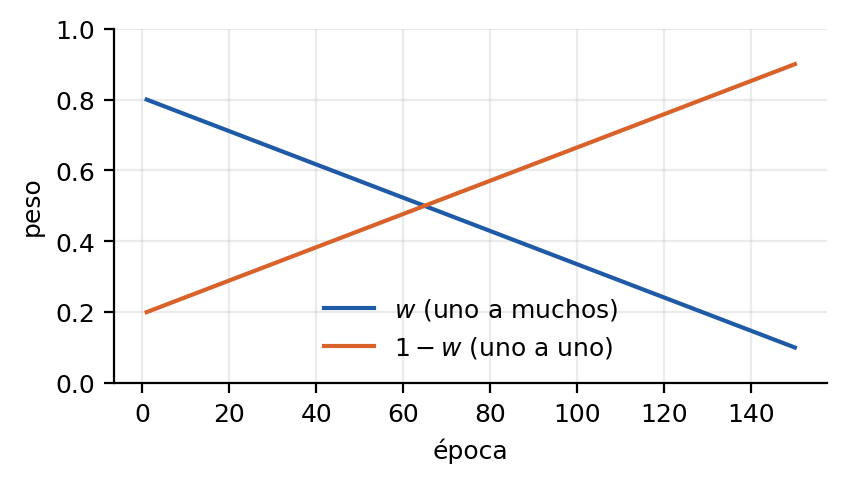
\includegraphics[width=0.62\textwidth]{progloss.png}
\caption{Peso de cada cabeza a lo largo de 150 épocas (ProgLoss).}
\label{fig:progloss}
\end{figure}

\begin{lstlisting}[style=py]
class PerdidaE2E:
    def __init__(self, nc, pasos, epocas, w0=0.8, wf=0.1):
        self.o2m = PerdidaCabeza(nc, pasos, topk=10)
        self.o2o = PerdidaCabeza(nc, pasos, topk=7, topk2=1)
        ...
    def fijar_epoca(self, e):
        self.w = max(1 - e / max(self.epocas - 1, 1), 0) * (self.w0 - self.wf) + self.wf
\end{lstlisting}

\begin{recuerda}
Recuerda el \cod{detach()} de la cabeza (capítulo~\ref{cap:arquitectura}): la
pérdida o2o solo entrena las capas propias de esa cabeza. La columna vertebral y
el cuello los entrena únicamente la o2m. Por eso la o2o puede volverse
«selectiva» sin estorbar a las características que comparten.
\end{recuerda}

\section{Detalles que importan}

\begin{itemize}
  \item La pérdida se calcula en \cod{float32} aunque la red corra en
        \cod{bfloat16} (precisión mixta): los logaritmos y las sumas grandes pierden
        precisión en 16 bits.
  \item Se multiplica por el tamaño del lote $B$ (como Ultralytics) para que la escala
        del gradiente no dependa de $B$ cuando se acumulan lotes.
  \item Si una imagen del lote no tiene objetos, solo contribuye a $L_{\text{clase}}$
        (todo es fondo). Si \emph{ningún} objeto del lote tiene celdas positivas,
        $L_{\text{caja}}$ y $L_{\text{dist}}$ valen cero pero siguen conectadas al
        grafo, así \cod{backward()} no falla.
\end{itemize}
